%\documentclass[12pt,aspectratio=169]{beamer}
%\input{../mybeamer}
%
\chapter{DC Circuit Analysis}
%\subtitle{AP Physics 2}
%\input{../me}
%\input{../mycommands}
%
%

%{Basic DC Circuit}
%  \begin{columns}
%    \column{.3\textwidth}
%    \centering
%    \begin{tikzpicture}[scale=1.8,american voltages,thick]
%      \draw (0,0) to[battery,l=$\mathcal E$] (0,1.5)--(1.5,1.5) to[R=$R$]
%      (1.5,0)--(0,0);
%    \end{tikzpicture}
%    
%    \column{.7\textwidth}
%    A basic circuits consists of:
%    \begin{itemize}
%    \item An energy source:
%      \begin{itemize}
%      \item Examples: battery, generator or capacitor
%      \item Creates a voltage gain, called the \textbf{electromotive force}, or
%        \emph{emf} ($\mathcal E$)
%      \end{itemize}
%    \item Loads:
%      \begin{itemize}
%        \item resistors, motor, LEDs
%      \end{itemize}
%    \item Connecting wires:
%      \begin{itemize}
%      \item Assume to have negligible resistance
%      \end{itemize}
%    \end{itemize}
%  
%
%
%
%
\section{Electric Current}
%
%{Electric Current}
%  In an electric circuit, a large number of charge ``carriers'' are pushed
%  along by a small electrostatic force in a conductive material, creating an
%  \textbf{electric current}. We can imagine positive charges moving from the
%  positive terminal towards the negative terminal.
%  \begin{center}
%    \begin{tikzpicture}[scale=.85,thick]
%      \fill[magenta!10] rectangle (7,3);
%      \draw[very thick] (0,0)--(7,0);
%      \draw[very thick] (0,3)--(7,3);
%      
%      \draw[fill=cyan!20] (1,.5) circle(.25) node{$+$};
%      \draw[axes] (1.25,.5)--(1.75,.5);
%
%      \draw[fill=cyan!20] (3,.75) circle(.25) node{$+$};
%      \draw[axes] (3.25,.75)--(3.75,.75);
%
%      \draw[fill=cyan!20] (6,1.75) circle(.25) node{$+$};
%      \draw[axes] (6.25,1.75)--(6.75,1.75);
%
%      \draw[fill=cyan!20] (5,2.5) circle(.25) node{$+$};
%      \draw[axes] (5.25,2.5)--(5.75,2.5);
%
%      \draw[fill=cyan!20] (4,1.75) circle(.25) node{$+$};
%      \draw[axes] (4.25,1.75)--(4.75,1.75);
%
%      \draw[fill=cyan!20] (5.25,1) circle(.25) node{$+$};
%      \draw[axes] (5.5,1)--(6,1);
%
%      \draw[fill=cyan!20] (2,1.5) circle(.25) node{$+$};
%      \draw[axes] (2.25,1.5)--(2.75,1.5);
%
%      \draw[fill=cyan!20] (.5,2.5) circle(.25) node{$+$};
%      \draw[axes] (.75,2.5)--(1.25,2.5);
%
%      \draw[fill=cyan!20] (2.5,2.25) circle(.25) node{$+$};
%      \draw[axes] (2.75,2.25)--(3.25,2.25);
%
%      \node at (0,1.5)[left] {\huge$+$};
%      \node at (7,1.5)[right]{\huge$-$};
%    \end{tikzpicture}
%  \end{center}
%  In a metal conductor, \textbf{charge carriers} are freely-moving electrons.
%  But in other applications protons or ions can also generate a current.
%
%
%
%
%\section{Electrical Current}
The average \textbf{electrical current} $I_\text{avg}$ through conductor is the
amount of charges $Q$ that passes through a point during a finite time interval
$\Delta t$:
\begin{equation}
  \boxed{
    I_\text{avg}=\frac Q{\Delta t}
  }
\end{equation}
Generally, the current through a conductor is a function of time ($I=I(t)$),
and $+/-$ signs may be used to indicate direction of the current.



\subsection{Direct Current}

In a \textbf{direct current} (\textbf{DC}), the flow of charges is always in
the same direction, but the current itself does not have to be constant in
time. The examples in Fig.~\ref{fig:DC-examples} of direct currents.
\begin{figure}[ht]
  \centering
  \begin{subfigure}{.28\textwidth}
    \centering
    \begin{tikzpicture}[scale=.85]
      \draw[red,ultra thick] (0,3)--(4,3);
      \draw[axes] (0,0)--(4,0) node[right]{$t$};
      \draw[axes] (0,0)--(0,4) node[above]{$I$};
    \end{tikzpicture}
    \caption{Resistive circuits}
  \end{subfigure}
  \begin{subfigure}{.34\textwidth}
    \centering
    \begin{tikzpicture}[scale=.85]
      \draw[smooth,samples=20,domain=0:3.5,functions]
      plot(\x,{3*(exp(-.8*\x))});
      \draw[axes] (0,0)--(4,0) node[right]{$t$};
      \draw[axes] (0,0)--(0,4) node[above]{$I$};
    \end{tikzpicture}
    \caption{Resistive \& capacitive circuits}
  \end{subfigure}
  \begin{subfigure}{.34\textwidth}
    \centering
    \begin{tikzpicture}[scale=.85]
      \draw[axes] (0,0)--(4,0) node[right]{$t$};
      \draw[axes] (0,0)--(0,4) node[above]{$I$};
      \draw[smooth,samples=20,domain=0:3.5,functions]
      plot(\x,{sin(120*\x)+2});
    \end{tikzpicture}
    \caption{Capacitive \& inductive circuits}
  \end{subfigure}
  \caption{Examples of direct-current circuits}
  \label{fig:DC-examples}
\end{figure}



\subsection{Alternating Current}

In an \textbf{alternating current} (\textbf{AC}), the flow of charges changes
in direction, \emph{usually} as a sinusoidal function of time.
\begin{figure}[ht]
  \centering
  \begin{subfigure}{.35\textwidth}
    \centering
    \begin{tikzpicture}[scale=.85]
      \draw[smooth,samples=50,domain=0:4,functions] plot(\x,{1.5*sin(150*\x)});
      \draw[axes] (0,0)--(5,0) node[right]{$t$};
      \draw[axes] (0,-2.5)--(0,2.5) node[above]{$I$};
    \end{tikzpicture}
  \end{subfigure}
  \begin{subfigure}{.35\textwidth}
    \centering
    \begin{tikzpicture}[scale=.85]
      \draw[smooth,samples=50,domain=0:4,functions] plot(\x,{1.5*sin(150*\x)});
      \draw[axes] (0,0)--(5,0) node[right]{$t$};
      \draw[axes] (0,-2.5)--(0,2.5) node[above]{$V$};
    \end{tikzpicture}
  \end{subfigure}
\end{figure}

The power outlet in North America are all AC, with a rms (root-mean-square)
voltage of \SI{120}\volt, and a frequency of \SI{60}\hertz.


%{Current Through the Conductor}
The expression for electric current can be expanded this way:

\begin{equation}
  I=\frac Q{\Delta t}=\left(\frac QV\right)\frac V{\Delta t}
  =\left[ne\right]\left[Av_d\right]
\end{equation}
where $Q/V$ is the \emph{amount of charges per volume}, which is also the
\textbf{charge carrier density} (number of charge carriers per volume) $n$
times the \textbf{elementary charge} $e$; $V/t$ is the rate the volume of
charges moves through the conductor, give by the cross-section area of the
conductor $A$ times the \textbf{drift velocity} $v_d$ of the charge carrier.

Calculating the charge carrier density in a \emph{metal} conductor involves
some physical information about the metal:
\begin{enumerate}
\item Divide the metal's density $\rho$ by its molar mass $M$ to find the
  \emph{number of moles of atoms per unit volume}
\item Multiply by Avogadro's number $N_A=\SI{6.0221e23}{\per mol}$ to find
  \emph{number of atoms per unit volume}
\item Multiply by the number of free electrons per atom $k$ for that
  particular metal
\end{enumerate}
Collecting all the terms from the last slide, we have:  
\begin{equation}
  \boxed{n=\frac{\rho kN_A}M}
\end{equation}
%%  \begin{center}
%%    \begin{tabular}{l|c|c}
%%      \rowcolor{pink}
%%      \textbf{Quantity} & \textbf{Symbol} & \textbf{SI Unit} \\ \hline
%%      Charge carrier density   & $n$    & \si{\per\metre\cubed} \\
%%      Density of material      & $\rho$ & \si{\kilo\gram\per\metre\cubed} \\
%%      Free electrons per atom  & $k$    & \\
%%      Avogadro's number        & $N_A$  & \si{\per\mol}\\
%%      Molar mass               & $M$    & \si{\kilo\gram\per\mol}
%%    \end{tabular}
%%  \end{center}
For copper, $M=\SI{63.54e-3}{\kilo\gram\per\mol}$,
$\rho=\SI{8.96e3}{\kilo\gram\per\metre\cubed}$, $k=1$ and therefore
$n=\SI{8.5e28}{\per\metre\cubed}$.
%%
%%
%%
%%
%%{Current}
%%  Another alternate description of the electric current is to express it in
%%  terms of the current density $J$, with a unit of of \emph{amp\`{e}re per
%%  meters squared} (\si{\ampere\per\meter\squared}).
%%  
%%  \begin{equation}
%%    \boxed{I=JA}
%%  }
%%
%%  It is obvious from the previous expression that the current density is the
%%  product of the charge carrier density, elementary charge, and the drift
%%  velocity:
%%
%%  \begin{equation}
%%    \boxed{J=nev_d}
%%  }
%%
%
%

\subsection{Modelling Electric Current}

\textbf{Conventional current} flows from the positive terminal (cathode) to the
negative terminal (anode). The flow  of current is assumed to be a continuous
function of time

We assume that positive charge carriers are all positively charged, and they
move with the same \textbf{drift velocity}. In most circuits, the drift
velocity is in the other of 0.1 to \SI1{\milli\metre\per\second}.

In reality, in a metal condcutor, electric current comes from motion of the
negatively-charged electrons moving in the \emph{opposite} direction of
convention current, called the \textbf{electron flow}, or
\textbf{electron current}, as shown in Fig.~\ref{fig:electron-flow}.
The electron's motion is chaotic, because as they move,
they collide with other electrons and with the atoms in the metal. The drift
velocity is the \emph{average} speed of the electrons. For circuit analysis,
we use the conventional current for simplicity.

\begin{figure}[ht]
  \centering
  \begin{subfigure}{.32\textwidth}
    \centering
    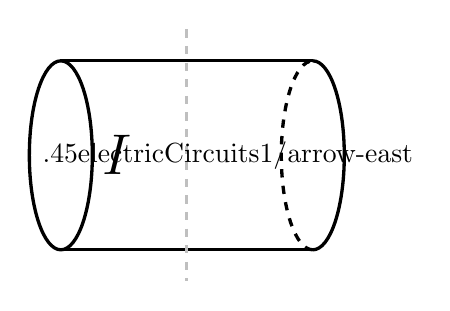
\begin{tikzpicture}[scale=.4]
      \draw[very thick] ellipse (1 and 3);
      \draw[very thick] (0,3)--+(8,0);
      \draw[very thick] (0,-3)--+(8,0);
      \draw[very thick] (8,-3) arc(-90:90:1 and 3);
      \draw[very thick,dashed] (8,-3) arc (270:90:1 and 3);
      \draw[very thick,dashed,lightgray] (4,4)--(4,-4);
      \node at (1.8,0){\huge$I$};
      \node at (5.3,0){\pic{.45}{electricCircuits1/arrow-east}};
    \end{tikzpicture}
    \caption{Electric current modelled as a continuously flow of charges}    
  \end{subfigure}
%    \end{center}
%    \vspace{-.1in}{\scriptsize\par
%    }
%    
%    \column{.34\textwidth}
%    \color{red}\begin{center}
%      Model: motion of (+) charges
  \begin{subfigure}{.32\textwidth}
    \centering
    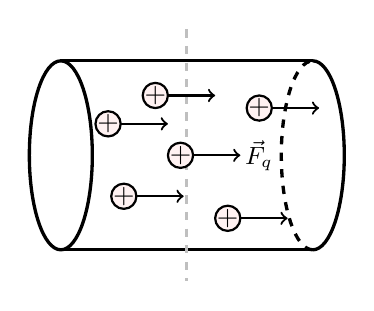
\begin{tikzpicture}[scale=.4]
      \draw[very thick] ellipse (1 and 3);
      \draw[very thick] (0,3)--+(8,0);
      \draw[very thick] (0,-3)--+(8,0);
      \draw[very thick] (8,-3) arc(-90:90:1 and 3);
      \draw[very thick,dashed] (8,-3) arc (270:90:1 and 3);
      \draw[very thick,dashed,lightgray] (4,4)--(4,-4);
        
      \draw[thick,fill=pink!20] (1.5,1) circle (.4) node{$+$};
      \draw[thick,->] (1.9,1)--+(1.5,0);

      \draw[thick,fill=pink!20] (2,-1.3) circle (.4) node{$+$};
      \draw[thick,->] (2.4,-1.3)--+(1.5,0);

      \draw[thick,fill=pink!20] (3,1.9) circle (.4) node{$+$};
      \draw[thick,->] (3.4,1.9)--+(1.5,0);

      \draw[thick,fill=pink!20] (3.8,0) circle (.4) node{$+$};
      \draw[thick,->] (4.2,0)--+(1.5,0) node[right=-2]{\small$\vec F_q$};

      \draw[thick,fill=pink!20] (5.3,-2) circle (.4) node{$+$};
      \draw[thick,->] (5.7,-2)--+(1.5,0);

      \draw[thick,fill=pink!20] (6.3,1.5) circle (.4) node{$+$};
      \draw[thick,->] (6.7,1.5)--+(1.5,0);
    \end{tikzpicture}
    \caption{Electric current modelled as the discrete motion of positive
      charges}
  \end{subfigure}
  \begin{subfigure}{.32\textwidth}
    \centering
    \begin{tikzpicture}[scale=.4]
      \draw[very thick] ellipse (1 and 3);
      \draw[very thick] (0,3)--+(8,0);
      \draw[very thick] (0,-3)--+(8,0);
      \draw[very thick] (8,-3) arc(-90:90:1 and 3);
      \draw[very thick,dashed] (8,-3) arc (270:90:1 and 3);
      \draw[very thick,dashed,lightgray] (4,4)--(4,-4);

      \draw[axes] (5,1)--(4,0)--(2.5,.5)--(.5,.8)--(0,0);
      \draw[thick,fill=pink!20] (5,1) circle (.4) node{\tiny$e^-$};

      \draw[axes] (8,-1)--(5,0)--(4.5,-.5)--(0,-.8); %--(0,0);
      \draw[thick,fill=pink!20] (8,-1) circle (.4) node{\tiny$e^-$};

      \draw[axes] (6.5,-1.8)--(4.2,-2)--(4,-1)--(2.5,-1.8)--(1,-1.5);
      \draw[thick,fill=pink!20] (6.5,-1.8) circle (.4) node{\tiny$e^-$};

      \draw[axes] (2.5,1.8)--(0,1.8);
      \draw[thick,fill=pink!20] (2.5,1.8) circle (.4) node{\tiny$e^-$};
    \end{tikzpicture}
    \caption{Electric current modelled as the discrete motion of negative
      charges}
    \label{fig:electron-flow}
  \end{subfigure}
  \caption{Modelling of electrical current}
\end{figure}


%{Conventional Current vs.\ Electron Flow}

%  We have \emph{assumed} that the charge carriers are positively charged, which
%  means that the current flows from high electric potential to low potential
%  (i.e.\ from cathode to anode).
%  \begin{center}
%    \begin{tikzpicture}[scale=.75]
%      \draw (0,0)--(10,0);
%      \draw (0,1)--(10,1) node[midway,above]{$I\longrightarrow$};
%      \foreach \x in {1,3,...,9}{
%        \draw[thick,fill=pink!40] (\x,.5) circle (.25) node{$+$};
%        \draw[thick,->] (\x+.25,.5)--(\x+.75,.5);
%      }
%    \end{tikzpicture}
%  \end{center}
%  In a conducting wire, instead of positive charges flowing in one direction,
%  we have, in fact, electrons (negative charges) flowing in the opposite
%  direction, called the :
%  \begin{center}
%    \begin{tikzpicture}[scale=.75]
%      \draw (0,0)--(10,0);
%      \draw (0,1)--(10,1) node[midway,above]{$I\longrightarrow$};
%      \foreach \x in {1,3,...,9}{
%        \draw[thick,fill=blue!40!gray!20] (\x,.5) circle (.25) node{$-$};
%        \draw[axes] (\x-.25,.5)--(\x-.75,.5);
%      }
%    \end{tikzpicture}
%  \end{center}
% 
%
%
%
\subsection{Electric Field Inside the Wire}
Inside the wire, there is a weak electric field, which exerts a force on the
free electrons as they move in the wire
\begin{itemize}
\item As the charges move through a conductor, they lose potential energy
\item Unlike a falling object which converts gravitational potential energy
  to kinetic energy, in a circuit, the energy is 
  \begin{itemize}
  \item converted into radiative heat or light through the resistance of the
    wire, or
  \item converted into kinetic energy of a motor shaft
  \end{itemize}
\end{itemize}



\section{Ohm's Law}

Georg Ohm discovered that when a current is passed through a piece of metal
conductor, the voltage (electric potential difference) $V$ across the two ends
of the metal is proportional to the amount of current ($I$) through it. This is
known as \textbf{Ohm's law}:
\begin{equation}
  \boxed{
    V=IR
  }
\end{equation}
The proportionality between voltage and current is called \textbf{resistance}.
We now know that electrical resistance is caused by the free electrons'
collisions with the atoms in the metal. The collisions transfer kinetic energy
from the electrons to the atoms. The atoms would then vibrate, and release
the additional energy in the form of electromagnetic radiation (as we have
learned, in Section~\ref{sec:heat-transfer}, is a form of heat transfer).
%The electric potential difference $V$ across a resistor equals the product of
%the current $I$ through the load and the resistance $R$:
%  \begin{center}
%    \begin{tabular}{l|c|c}
%      \rowcolor{pink}
%      \textbf{Quantity} & \textbf{Symbol} & \textbf{SI Unit} \\ \hline
%      Potential difference & $V$    & \si\volt \\
%      Current              & $I$    & \si\ampere \\
%      Resistance           & $R$    & \si\ohm
%    \end{tabular}
%  \end{center}
%  A load is considered ``ohmic'' if it obeys Ohm's law.
Note that Ohm's law is \emph{not} a fundamental law in physics; it only applies
to mostly metal conductors.

Electrical devices where the relationship between voltage across the device and
the current through the device is linear are called \textbf{ohmic devices}.
Incandescent light bulbs and heating elements are examples of ohmic devices.
If we plot the current vs.\ voltage for the device, we would find a straight
line; the slope of the graph is the inverse of the resistance, as shown in
Fig.~\ref{fig:ohmic-relationship}.
\begin{figure}[ht]
  \centering
  \begin{subfigure}{.32\textwidth}
    \centering
    \begin{tikzpicture}
      \draw[functions] (0,0)--(2.5,2.5)
      node[midway,right]{$\text{slope}=\dfrac1R$};
      \draw[axes] (0,0)--(3,0) node[right]{$V$};
      \draw[axes] (0,0)--(0,3) node[right]{$I$};
    \end{tikzpicture}
    \caption{Ohmic}
    \label{fig:ohmic-relationship}
  \end{subfigure}
  \begin{subfigure}{.32\textwidth}
    \centering
    \begin{tikzpicture}
      \draw[axes] (0,0)--(3,0) node[right]{$V$};
      \draw[axes] (0,0)--(0,3) node[right]{$I$};
      \draw[functions,domain=0:2.45,smooth] plot(\x,.0008*\x^9);
    \end{tikzpicture}
    \caption{Non-ohmic}
    \label{fig:non-ohmic-relationship}
  \end{subfigure}
  \caption{Relationship between current and voltage for ohmic and non-ohmic
    devices.}
  \label{fig:i-vs-v-diagrams}
\end{figure}
Loads that are \textbf{non-ohmic} do not obey Ohm's law; the relationship
between voltage and current is \emph{not} linear, as shown in
Fig.~\ref{fig:non-ohmic-relationship}. Semi-conductor devices such as diodes
(e.g.\ your TV's LED screen) are non-ohmic. As well, a DC motor is only ohmic
if it is stalled (i.e.\ when current passes through the current but the motor
shaft is not turning).
\begin{remark}
  For clarification, in the graphs in Fig.~\ref{fig:i-vs-v-diagrams}, we have
  plotted $I$ vs.\ $V$. This is because we usually alter the voltage as an
  \emph{input}, and then measure the resulting current in the circuit as an
  \emph{output}. From this point of view, it makes sense that $V$ is the
  independent variable, and $I$ is the dependent variable. You can, of course,
  reverse the axes by plotting $V$ vs.\ $I$. In this case, across an ohmic
  device, the line would still be straight, but the slope would now be the
  resistance $R$.
\end{remark}



\subsection{Resistance of a Conductor}

The resistance of a conductor is proportional to the resistivity $\rho$ and
its length $L$, and inversely proportional to the cross-sectional area $A$:
\begin{equation}
  \boxed{
    R=\rho\frac LA
  }
\end{equation}
%  \begin{center}
%    \begin{tabular}{l|c|c}
%      \rowcolor{pink}
%      \textbf{Quantity} & \textbf{Symbol} & \textbf{SI Unit} \\ \hline
%      Resistance           & $R$    & \si\ohm \\
%      Resistivity          & $\rho$ & \si{\ohm\metre}\\
%      Length of conductor  & $L$    & \si\metre \\
%      Cross-sectional area & $A$    & \si{\metre\squared}
%    \end{tabular}
%  \end{center}
The resistivity $\rho$ is a material property, which is usually determined
experimentally. The SI unit for resistivity is an \textbf{ohm metre}
(\si{\ohm\metre}).
\begin{table}[ht]
  \centering
  \begin{tabular}{c|c}
    \rowcolor{pink!50}
    Material & Resistivity $\rho$ (\si{\ohm\metre})\\ \hline
    silver & \num{1.6e-8} \\
    copper    & \num{1.7e-8} \\
    aluminum  & \num{2.7e-8} \\
    tungsten  & \num{5.6e-8} \\
    Nichrome  & \num{100e-8} \\
    carbon    & \num{3500e-8}\\
    germanium & \num{.46} \\
    glass     & \num{e10} to \num{e14}\\
  \end{tabular}
  \caption{Resistivity of common materials}
\end{table}

Resistivity of a material is also the ratio between strength of the electric
field $E$ inside the material (the electric field that drives the current)
and the current density $J$:
\begin{equation}
  \boxed{
    \rho=\frac EJ
  }
\end{equation}
%  \begin{itemize}
%  \item Conductor: the electrons are free to move, therefore the electric
%    field tend to be very small, and the resistivity is low.
%  \item Insulators and dielectric: electrons cannot move easily (dielectric:
%    they can only polarize themselves) the electric field are generally
%    strong, and the resistivity is higher.
%  \end{itemize}
%



%{Resistance of a Conductor}
%
%  \eq{.0in}{
%    \boxed{R=\rho\frac LA}
%  }
%  

%    \centering
%    \begin{tabular}{c|c|c}
%      \rowcolor{blue!50}
%               {\color{white}Gauge} & 
%               {\color{white}Diameter} & 
%               {\color{white}$R/L$} \\
%               \rowcolor{blue!50}
%        & {\color{white}(\si{\milli\metre})} & 
%                        {\color{white}(\SI{e-3}{\ohm\per\metre})}\\ \hline
%                        0  & \num{9.35} & \num{0.31} \\
%                        10 & \num{2.59} & \num{2.20} \\
%                        14 & \num{1.63} & \num{8.54} \\
%                        18 & \num{1.02} & \num{21.90} \\
%                        22 & \num{0.64} & \num{51.70} \\
%    \end{tabular}




\subsection{Power Dissipated by a Load}
Average power $P$ is the rate at which work $W$ is done, and from
electrostatics, the change in electric potential energy $\Delta E_q$ is
proportional to the amount of charge $q$ and the voltage $V$. This gives a
very simple expression for power through a resistor:
\begin{equation}
  P=\frac W{\Delta t}=\frac{\Delta (qV)}{\Delta t}
  =\left(\frac{\Delta q}{\Delta t}\right)V
  \;\rightarrow\;\boxed{P=IV}
\end{equation}
%  \begin{center}
%    \begin{tabular}{l|c|c}
%      \rowcolor{pink}
%      \textbf{Quantity} & \textbf{Symbol} & \textbf{SI Unit} \\ \hline
%      Power through a load    & $P$ & \si\watt \\
%      Current through a load  & $I$ & \si\ampere \\
%      Voltage across the load & $V$ & \si\volt
%    \end{tabular}
%  \end{center}
This relationship applies regardless of whether the loads are ohmic or not
%
%
%
%
%{Other Equations for Power}
Combining Ohm's law ($V=IR$) with power equation, we get two additional
expressions for power through a resistor:
\begin{equation}
  \boxed{P=\frac{V^2}R}\quad\quad\boxed{P=I^2R}
\end{equation}
%  \begin{center}
%    \begin{tabular}{l|c|c}
%      \rowcolor{pink}
%      \textbf{Quantity} & \textbf{Symbol} & \textbf{SI Unit} \\ \hline
%      Power      & $P$ & \si\watt \\
%      Voltage    & $V$ & \si\volt \\
%      Resistance & $R$ & \si\ohm  \\
%      Current    & $I$ & \si\ampere
%    \end{tabular}
%  \end{center}
Not surprisingly, these equations will only apply to ohmic devices.



\section{Other Circuit Devices}

Aside from the necessary circuit devices,

For example, an energy sources may include:
\begin{figure}[ht]
  \centering
  \begin{subfigure}{.32\textwidth}
    \centering
    \begin{tikzpicture}[american voltages,thick]
      \draw (0,0) to[battery1,o-o] (2,0);
    \end{tikzpicture}
    \caption{A voltaic cell}
  \end{subfigure}
  \begin{subfigure}{.32\textwidth}
    \centering
    \begin{tikzpicture}[american voltages,thick]
      \draw (0,0) to[battery,o-o] (2,0);
    \end{tikzpicture}
    \caption{A voltaic pile (battery)}
  \end{subfigure}
  \begin{subfigure}{.32\textwidth}
    \centering
    \begin{tikzpicture}[american voltages,thick]
      \draw (0,0) to[pvsource,o-o] (2,0);
    \end{tikzpicture}
    \caption{A solar panel}
  \end{subfigure}

  \begin{subfigure}{.32\textwidth}
    \centering
    \begin{tikzpicture}[american voltages,thick]
      \draw (0,0) to[C,o-o] (2,0);
    \end{tikzpicture}
    \caption{A capacitor}
  \end{subfigure}
  \begin{subfigure}{.32\textwidth}
    \centering
    \begin{tikzpicture}[american voltages,thick]
      \draw (0,0) to[american voltage source,o-o] (2,0);
    \end{tikzpicture}
    \caption{A DC voltage source}
  \end{subfigure}
  \begin{subfigure}{.32\textwidth}
    \centering
    \begin{tikzpicture}[american voltages,thick]
      \draw (9,0) to[sinusoidal voltage source,o-o] (11,0);
    \end{tikzpicture}
    \caption{An AC voltage source}
  \end{subfigure}
\end{figure}

A \textbf{capacitor} can also act as a energy source. When a capacitor is
charged---with charge $+Q$ on one plate, and $-Q$ on the other, a voltage is
generated, according to the equation $V=Q/C$ (studied in
Chapter~\ref{chapter:capacitor}).
%  \begin{center}
%    \begin{tikzpicture}[thick]
%      \draw (3,0) to[C,l=Capacitor,o-o] (5,0);
%    \end{tikzpicture}
%  \end{center}
%  Circuits with both resistors and capacitors will be studied next class.

There are also other circuit devices that are not strictly necessary, but are
very important/useful to ensure the reliable operation of an electrical
circuit. For examples:
\begin{figure}[ht]
  \centering
  \begin{tikzpicture}[thick,scale=1.2]
    \draw (0,0) to[fuse,l=Fuse,o-o] (2,0);
  \end{tikzpicture}
  \caption{Circuit diagram of a fuse}  
\end{figure}

Loads are devices that transforms the electrical energy in the circuit into
other forms of energy. Examples include:
\begin{figure}[ht]
  \centering
  \begin{subfigure}{.24\textwidth}
    \centering
    \begin{circuitikz}[american voltages]
      \draw[thick] (0,0) to[R,o-o] (2,0);
    \end{circuitikz}
    \caption{Resistor}
  \end{subfigure}
  \begin{subfigure}{.24\textwidth}
    \centering
    \begin{circuitikz}[american voltages]
      \draw[thick] (3,0) to[bulb,o-o] (5,0);
    \end{circuitikz}
    \caption{Light bulb}
  \end{subfigure}
  \begin{subfigure}{.24\textwidth}
    \centering
    \begin{circuitikz}[american voltages]
      \draw[thick] (6,0) to[lamp,o-o] (8,0);
    \end{circuitikz}
    \caption{Lamp}
  \end{subfigure}
  \begin{subfigure}{.24\textwidth}
    \centering
    \begin{circuitikz}[american voltages]
      \draw[thick] (9,0) to[short,o-o] (11,0);
       \draw[very thick,fill=white] (9.35,-.2) rectangle (10.65,.2);
       \draw[very thick,fill=white] (10,0) circle (14pt) node{M};
    \end{circuitikz}
    \caption{DC motor}
  \end{subfigure}
\end{figure}
%  \begin{itemize}
%    \item Resistors, light bulbs and other lamps transform electrical energy
%      into heat, light and other forms of
%      \textbf{electromagnetic radiation}\footnote{Also known as
%      \textbf{electromagnetic waves}, or \textbf{EM waves}. They include radio
%      waves, microwaves, infrared radiation, visible light, ultraviolet (UV)
%      radiation, x-ray and gamma rays}
%    \item A motor converts electrical energy into kinetic energy of the motor
%      shaft and whatever objects are connected to it through an interaction
%      with a magnetic field inside the motor
%  \end{itemize}





A \textbf{fuse} will break (stopping current from flowing) when the current
through it exceeds its rating.

\begin{figure}[ht]
  \centering
  \begin{tikzpicture}[thick]
    \draw (0,0) to[short,o-] (.7,0) to[short,-*]
    +({.6*cos(40)},{.6*sin(40)});
    \draw (1.3,0) to[short,*-o] (2,0);
    \node at (1,.8){Switch};
  \end{tikzpicture}
\end{figure}
A switch allows the circuit to be manually turned on or off. (In the example,
the switch is open and no current flows through it.)



\section{Measuring Devices}

A \textbf{voltmeter} (Fig.~\ref{fig:voltmeter}) is used to measure the voltage
across two points in a circuit. To measure the voltage across a load, it is
placed in \emph{parallel} with a load. % to measure the voltage across it.
An ideal voltmeter has infinite resistance ($R=\infty$) and no current through
it ($I=0$).

An \textbf{ammeter} (Fig.~\ref{fig:ammeter}) is used to measure the current
across a point in the circuit. It is placed in \emph{series} with a load to
measure the current through it. An ideal ammeter has zero resistance ($R=0$),
thus it does not alter the flow of current in the circuit

An \textbf{ohmmeter} is used to measure the resistance of a particular load.
It is placed in \emph{parallel} with a load.
%to measure  the resistance across the load.
It can only be used when there is no active current in the circuit.
\begin{figure}[ht]
  \centering
  \begin{subfigure}{.32\textwidth}
    \centering
    \begin{tikzpicture}[scale=1.5]
      \draw[thick] (.2,0) to[R,l=$R$] (2.8,0);
      \draw[thick] (.7,0) to[short,*-](.7,-.8)--(2.3,-.8) to[short,-*] (2.3,0);
      \draw[very thick,fill=black!2] (1.5,-.8) circle (.3) node{V};
    \end{tikzpicture}
    \caption{Voltmeter}
    \label{fig:voltmeter}
  \end{subfigure}
  \begin{subfigure}{.32\textwidth}
    \centering
    \begin{tikzpicture}[scale=1.5]
      \draw[thick] (0,0) to[short] (1,0) to[R,l=$R$] (2.8,0);
      \draw[very thick,fill=black!2] (.7,0) circle (.3) node{A};
    \end{tikzpicture}
    \caption{Ammeter}
    \label{fig:ammeter}
  \end{subfigure}
  \begin{subfigure}{.32\textwidth}
    \centering
    \begin{tikzpicture}[scale=1.5]
      \draw[thick] (0,0) to[R,l=$R$] (3,0);
      \draw[thick] (.7,0) to[short,*-] (.7,-.8)--(2.3,-.8) to[short,-*](2.3,0);
      \draw[very thick,fill=black!2] (1.5,-.8) circle (.3) node{$\Omega$};
    \end{tikzpicture}
    \caption{Ohmmeter}
  \end{subfigure}
\end{figure}

Voltmeters, ammeters and ohmmeters operate on the same principle using magnetic
effects inside the device, called a \textbf{galvanometer}. Modern voltmeters
are usually part of a \textbf{multi-meter} that also operates as an ammeter
and ohmmeter.
\begin{figure}[ht]
  \centering
  \pic{.4}{electricCircuits1/voltmeter}
\end{figure}



\section{Kirchhoff's Laws}
%
\subsection{Kichhoff's Junction Law}
In the \textbf{junction law}, also known as the \textbf{current law}, the
electrical current that flows into any junction in a circuit must be equal to
the current which flows out.

\begin{figure}[ht]
  \centering
  \begin{tikzpicture}[scale=1.2]
    \draw[thick] (1,1) to[short,o-*] (1,0)--(0,0)--(0,-.7) to[R] (0,-2);
    \draw[thick] (1,-2) to[C] (1,-.7)--(1,0)--(2,0)--(2,-.7) to[L] (2,-2);
    \begin{scope}[ultra thick,red,->]
      \draw (1,.9)--(1,.1) node[midway,right]{$I$};
      \draw (.9,0)--(.1,0) node[midway,above]{$I_1$};
      \draw (1,-.1)--(1,-.9) node[midway,right]{$I_2$};
      \draw (1.1,0)--(1.9,0) node[midway,above]{$I_3$};
    \end{scope}
  \end{tikzpicture}
  \caption{An example of the junction law}
  \label{fig:junction-law}
\end{figure}
In the example in Fig.~\ref{fig:junction-law}, there are 4 paths to the
junction at the centre, with $I$ flowing into the junction, and $I_1$, $I_2$,
$I_3$ flowing out, then the junction law says that
\begin{equation*}
  I=I_1+I_2+I_3
\end{equation*}
regardless of what circuit devices those paths are connected to. In the
example, a resistor, a capacitor and an inductor\footnote{Inductor coils usee
magnetic field inside a solenoid to storage energy. It is \emph{not} part of
AP Physics 2} are joined at the junction. The junction law implies that there
must be no accumulation of charges anywhere in the circuit.



\subsection{Kichhoff's Voltage Law}

In the \textbf{voltage law}, the voltage changes around any closed loop in
the circuit must sum to zero, no matter what path you take through an
electrical circuit. In the example in Fig.~\ref{fig:voltage-law}, voltage gains
and losses from any of the loops always sum to zero:
\begin{align*}
  +\mathcal E-V_1-V_2 &= 0\quad\text{(ABCHA)}\\
  +\mathcal E-V_1-V_C &= 0\quad\text{(ABCDGHA)}\\
  +\mathcal E-V_1-V_L &=0\quad\text{(ABCDEFGHA)}
\end{align*}

\begin{figure}[ht]
  \centering
  \begin{tikzpicture}[scale=1.55,american voltages,thick]
    \draw (0,0) to[battery,l=$\mathcal E$] (0,1.5) to [R=$R_1$] (1.5,1.5)
    to[R=$R_2$] (1.5,0)--(0,0);
    \draw (1.5,1.5)--(2.5,1.5) to[C=$C$] (2.5,0)--(1.5,0);
    \draw (2.5,1.5)--(3.5,1.5) to[L=$L$] (3.5,0)--(2.5,0);
    \fill circle (.04) node[below left]{$A$};
    \fill (0,1.5) circle (.04) node[above left]{$B$};
    \fill (1.5,1.5) circle (.04) node[above]{$C$};
    \fill (2.5,1.5) circle (.04) node[above]{$D$};
    \fill (3.5,1.5) circle (.04) node[above]{$E$};
    \fill (3.5,0) circle (.04) node[below]{$F$};
    \fill (2.5,0) circle (.04) node[below]{$G$};
    \fill (1.5,0) circle (.04) node[below]{$H$};
  \end{tikzpicture}
  \caption{An example circuit with many elements}
  \label{fig:voltage-law}
\end{figure}


%%
%%    If I incorrectly guess that $I$ flows counterclockwise, I
%%    will still have a similar expression
%%
%%    \begin{equation}
%%      -V_R-V=0\;\;\rightarrow\;\; -V-IR=0
%%    }
%  
%  \vspace{.1in}This applies regardless of what devices (e.g.\ batteries,
%  resistors, capacitors, inductors, motors) are in the circuit.
%%  When solving for $I$, we get a negative number, indicating
%%  that my guess was in the wrong direction.
%
%
%
%
%{Kichhoff's Voltage Law}
%  

%    \centering
%    \begin{tikzpicture}[scale=1.75,american voltages,thick]
%      \draw (1,1.5) to[short,o-] (1.5,1.5) to[R=$R_2$] (1.5,0)
%      to[short,-o] (1,0);
%      \draw (1.5,1.5)--(2.5,1.5) to[C=$C$] (2.5,0)--(1.5,0);
%      \draw (2.5,1.5)--(3.5,1.5) to[L=$L$] (3.5,0)--(2.5,0);
%    \end{tikzpicture}
%    
%    \column{.6\textwidth}
The voltage law can also show that the voltage across any circuit devices
connected in parallel (side by side) must be the same:
%    
%    \begin{equation}
%      V_2=V_C=V_L
%    }
%%
%%    If I incorrectly guess that $I$ flows counterclockwise, I
%%    will still have a similar expression
%%
%%    \begin{equation}
%%      -V_R-V=0\;\;\rightarrow\;\; -V-IR=0
%%    }
%  
%
%
%
%
\section{Resistors in Circuits}

\subsection{Resistors in Parallel}

\begin{figure}[ht]
  \centering
  \begin{tikzpicture}[thick]
    \draw (0,2)  to[short,o-] (1,2) to[R=$R_1$] (1,0) to[short,-o] (0,0);
    \draw (1,2)  to[short] (2.25,2) to[R=$R_2$] (2.25,0) to[short] (1,0);
    \draw (2.25,2) to[short] (3.5,2) to[R=$R_3\ldots$] (3.5,0)
    to[short] (2.25,0);
  \end{tikzpicture}
  \caption{Circuit diagram of 3 resistors connected in parallel}
\end{figure}
From the current law, we know that the total current is the current through all
the resistors, which we can rewrite in terms of voltage and resistance using
Ohm's law:
%
%    \begin{equation}
%      I=I_1+I_2+I_3\cdots=\frac{V_1}{R_1}+\frac{V_2}{R_2}+\frac{V_3}{R_3}\cdots
%    }
    
But since we also know that $V_1=V_2=V_3=\cdots=V$ from the voltage law, we
can re-write as
\begin{equation*}
  I=\frac V{R_p}=V\left(\frac1{R_1}+\frac1{R_2}+\frac1{R_3}\cdots\right)
\end{equation*}
The equivalent resistance of a parallel circuit can found by applying Ohm's law
and Kirchhoff's laws: The inverse of the equivalent resistance is the sum of
the inverses of the individual resistances.
\begin{equation}
  \boxed{
    \frac1{R_p}=\sum_i\frac1{R_i}
  }
\end{equation}
%  \begin{center}
%    \begin{tabular}{l|c|c}
%      \rowcolor{pink}
%      \textbf{Quantity} & \textbf{Symbol} & \textbf{SI Unit} \\ \hline
%      Equivalent resistance in parallel & $R_p $ & \si\ohm \\
%      Resistance of individual loads    & $R_i $ & \si\ohm
%    \end{tabular}
%  \end{center}
Increasing the number of resistors in parallel \emph{decreases} $R_p$ because
it effectively increases the cross section area that the current passes through.

%    \begin{tikzpicture}[thick]
%      \draw (0,0) to[R=$R$,o-o] (3,0);
%    \end{tikzpicture}
%
%    \vspace{.6in}$R_\text{eq}=R$
%    
%    \centering
%
%    \vspace{.2in}
%    \begin{tikzpicture}[thick]
%      \draw (0,0) to[short,o-] (.3,0)--(.3,.7) to[R=$R$] (2.7,.7)--(2.7,0)
%      to[short,-o] (3,0);
%      \draw (.3,0)--(.3,-.7) to[R=$R$] (2.7,-.7)--(2.7,0);
%    \end{tikzpicture}
%    
%    \vspace{.27in}$R_\text{eq}=\dfrac R2$
%    
%    \begin{tikzpicture}[thick]
%      \draw (0,0) to[R=$R$,o-o] (3,0);
%      \draw (.3,0)--(.3,1.2) to[R=$R$] (2.7,1.2)--(2.7,0);
%      \draw (.3,0)--(.3,-1.2) to[R=$R$] (2.7,-1.2)--(2.7,0);
%    \end{tikzpicture}
%
%    \vspace{.1in}$R_\text{eq}=\dfrac R3$
%  
%  \vspace{.1in}The parallel equivalent resistance is \emph{always} lower than
%  the lowest resistor.
%
%
%
%
\subsection{Resistors in Series}
\begin{figure}[ht]
  \centering
  \begin{tikzpicture}[thick]
    \draw (0,0) to[R=$R_1$,o-] (2,0) to[R=$R_2$] (4,0) to[R=$R_3$,-o] (6,0);
  \end{tikzpicture}
  \caption{Circuit diagrams of 3 resistors connected in series}
\end{figure}
The analysis for resistors in series is similar (but easier). The current
through each resistor is the same:
%  \eq{-.2in}{
%    I_1=I_2=I_3=\cdots=I
%  }
And the total voltage drop across all resistor is therefore:
%  \begin{equation}
%    V=V_1+V_2+V_3+\cdots=I(\underbrace{R_1+R_2+R_3+\cdots}_{R_s})
%  }
%
%
%
%
%{Equivalent Resistance in Series}
Again, by applying Ohm's law and Kirchhoff's laws, we can find the equivalent
resistance ($R_s$) in series: it is the sum of the resistances of the
individual loads ($R_i$):
\begin{equation}
  \boxed{R_s=\sum_iR_i}
\end{equation}
Increasing the number of resistors in parallel \emph{increases} $R_s$ because
it effectively increases the length of the resistor that the current passes
through.
%
%
%
\section{Combination Circuits}
%{Tips for Solving ``Simple'' Circuit Problems}
\begin{enumerate}
\item Identify groups of resistors that are in parallel or in series, and
  find their equivalent resistance.
\item Gradually reduce the entire circuit to one voltage source and one
  resistor.
\item Using Ohm's law, find the current out of the battery.
\item Using Kirchhoff's laws, find the current through each of the resistors.
\end{enumerate}




\section{Internal Resistance}

%{Internal Resistance, Electromotive Force, Terminal Voltage}
\textbf{Internal Resistance:}
\begin{itemize}
\item The resistance within the battery itself
\item Analogy: like the friction inside an engine itself. Some energy is
  needed to overcome that friction
\end{itemize}
\textbf{Electromotive Force} (\emph{emf} or $\mathcal E$)
\begin{itemize}
\item The part of battery that actually provides the energy source
\item Not an actual ``force'' as we understand it (think energy instead)
\item Without internal resistance, terminal voltage = $\mathcal E$
\end{itemize}
%
%
%
%
%{Terminal Voltage and \emph{emf}}
The terminal voltage (or potential difference across the poles) of a battery
is the difference of the emf ($\mathcal E$) of the battery and the potential
drop across the internal resistance of the battery.
\begin{equation}
  \boxed{V_S = \mathcal{E}-V_\text{int}}
\end{equation}
%  \begin{center}
%    \begin{tabular}{l|c|l}
%      \rowcolor{pink}
%      \textbf{Quantity} & \textbf{Symbol} & \textbf{SI Unit} \\ \hline
%      Terminal voltage & $V_S$ & \si\volt \\
%      Electromotive force & $\mathcal E$ & \si\volt \\
%      Internal potential drop of a battery & $V_\text{int}$ & \si\volt
%    \end{tabular}
%  \end{center}
If no current passes through a battery, then the potential difference across
the internal resistance will be zero ($V_\text{int}=0$)

\begin{example}
  A battery with an \emph{emf} of \SI{9.0}{\volt} has an internal resistance of
  \SI{.0500}\ohm. Calculate the potential difference lost to the internal
  resistance, and the terminal voltage of the battery, if it is connected to an
  external resistance of \SI{4.00}\ohm.
\end{example}
